\documentclass[11pt]{article}

\usepackage{acronym}
\usepackage{graphicx}

\AddToHook{cmd/section/before}{\clearpage}

\begin{document}

%%% --- placeholderes --- %%%

\newcommand{\XX}{\textcolor{red}{XX}\xspace}


%%% --- formatting --- %%%

\newcommand{\crefrangeconjunction}{--}


%%% --- special terms --- %%%

\newcommand{\code}[1]{{\fontfamily{pcr}\selectfont\small #1}\xspace}
\newcommand{\ligocam}{\code{ligocam}}
\newcommand{\pemcoupling}{\code{pemcoupling}}
\newcommand{\pygrb}{\code{pyGRB}}
\newcommand{\xpip}{\code{X-pipeline}}
\newcommand{\reg}{\textsuperscript{\textregistered}}


%%% --- units --- %%%

\newcommand{\hyp}{\nobreakdashes-}
\newcommand{\meter}{\mathrm{m}\xspace}
\newcommand{\rthz}{\mathrm{Hz}^{1/2}\xspace}
\newcommand{\msol}{M_{\odot}\xspace}


%%% --- math and signal processing --- %%%

\newcommand{\bkg}{_{\textrm{bkg}}}
\newcommand{\inj}{_{\textrm{inj}}}
\newacro{ASD}{amplitude spectral density}
\newacroplural{ASD}[ASDs]{amplitude spectral densities}
\newacro{PSD}{power spectral density}
\newacroplural{PSD}[PSDs]{power spectral densities}
\newacro{RF}{radio-frequency}
\newacro{SNR}{signal-to-noise ratio}
\newacro{ADC}{analog-to-digital converter}
\newacro{DAC}{digital-to-analog converter}

%%% --- acronyms --- %%%

% general acronyms
\newacro{LIGO}{Laser Interferometer Gravitational-Wave Observatory}
\newacro{iLIGO}{Initial LIGO}
\newacro{aLIGO}{Advanced LIGO}
\newacro{LISA}{Laser Interferometer Space Antenna}
\newacro{O1}{the first observing run}
\newacro{O2}{the second observing run}
\newacro{O3}{the third observing run}
\newacro{O4}{the fourth observing run}

% detector jargon
\newacro{DARM}{differential arm length measurement}
\newacro{ETM}{end test mass}
\newacro{HAM}{horizontal access module}
\newacro{HVAC}{heating, ventilation, and air conditioning}
\newacro{IMC}{input mode cleaner}
\newacro{ITM}{input test mass}
\newacro{LHO}{LIGO Hanford Observatory}
\newacro{LLO}{LIGO Livingston Observatory}
\newacro{OMC}{output mode clearner}
\newacro{PEM}{physical environmental monitoring}
\newacro{PSL}{pre-stabilized laser}
\newacro{WFS}{wavefront sensor}

% astrophysics jargon
\newacro{GW}{gravitational wave}
\newacro{GRB}{gamma-ray burst}
\newacro{CBC}{compact binary coalescence}
\newacro{BH}{black hole}
\newacro{NS}{neutron star}
\newacroindefinite{NS}{an}{a}
\newacro{BBH}{binary black hole}
\newacro{NSBH}{neutron star-black hole}
\newacroindefinite{NSBH}{an}{a}
\newacro{BNS}{binary neutron star}
\newacroplural{BNS}[BNSs]{neutron star binaries}
\newacroplural{BBH}[BBHs]{black hole binaries}
\newacroplural{NSBH}[NSBHs]{neutron star-black hole binaries}
\newacro{ADI}{accretion disk instability}
\newacro{CSG}{circular sine-Gaussian}
\newacro{GBM}{Gamma-ray Burst Monitor}
\newacro{BAT}{Burst Alert Telescope}
\newacro{GCN}{Gamma-ray Coordinates Network}
\newacro{CMB}{cosmic microwave background}
\newacro{SN}{supernova}
\newacroplural{SN}[SNe]{supernovae}
\newacro{CCSN}{core-collapse supernova}
\newacroplural{CCSN}[CCSNe]{core-collapse supernovae}
\newacro{CSG}{circular sine-Gaussian}
\newacro{ADI}{accretion disk instability}

% searches
\newacro{cWB}{coherent waveburst}

% misc jargon
\newacro{DQR}{Data Quality Report}
\newacro{RC}{reaction chain}


\section{Chapter 1}

\begin{figure}[h!]
	\centering
	% \includegraphics[width=\textwidth]{figures/gw_polarization.png}
	\caption{
		The PEM system layout at LLO during O3, as seen on the PEM public website.}
	\label{fig:gw_polarization}
\end{figure}

\begin{figure}[h!]
	\centering
	% \includegraphics[width=\textwidth]{figures/gw_detector.png}
	\caption{
		Schematic of a simple Michelson interferometer designed for GW}
	\label{fig:gw_polarization}
\end{figure}

\section{Chapter 2}

\section{Chapter 3}

\begin{figure}[h!]
	\centering
	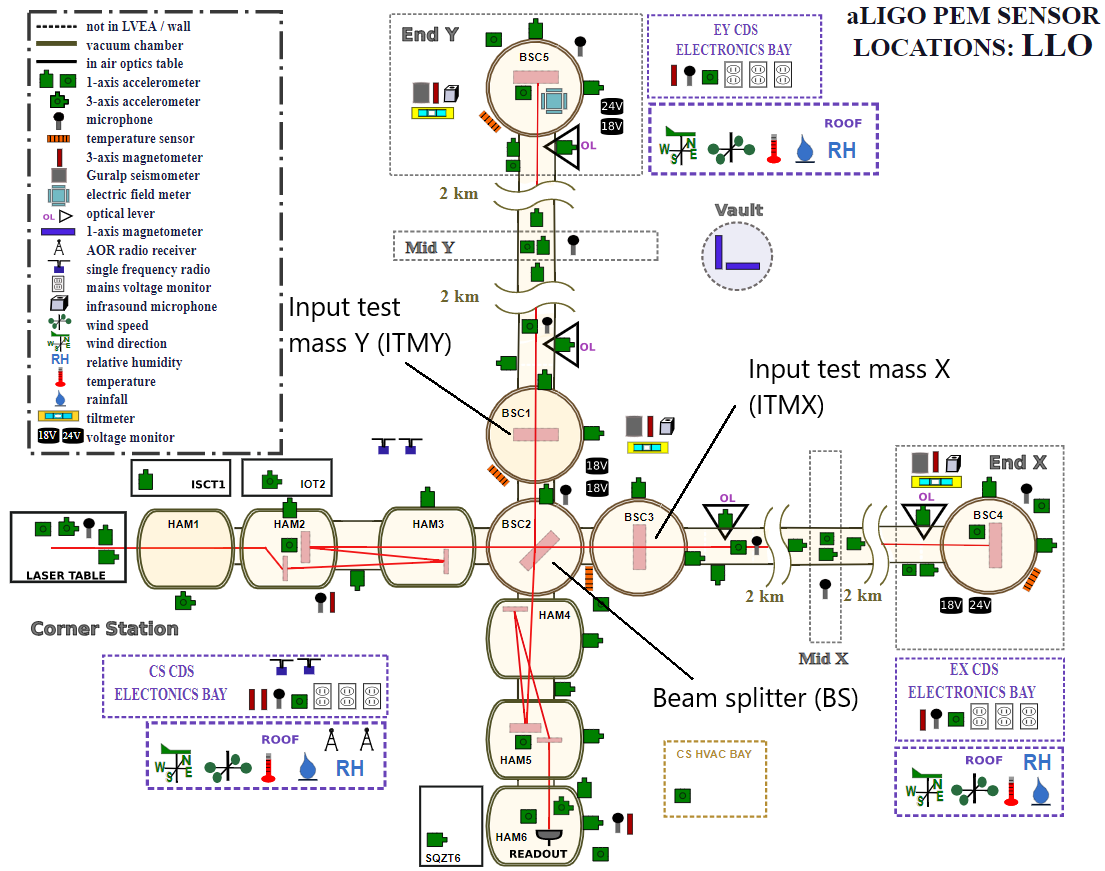
\includegraphics[width=\textwidth]{figures/pem-channels.png}
	\caption{
		The PEM system layout at LLO during O3, as seen on the PEM public website.}
	\label{fig:pem_channels}
\end{figure}

\begin{figure}[h!]
	\centering
	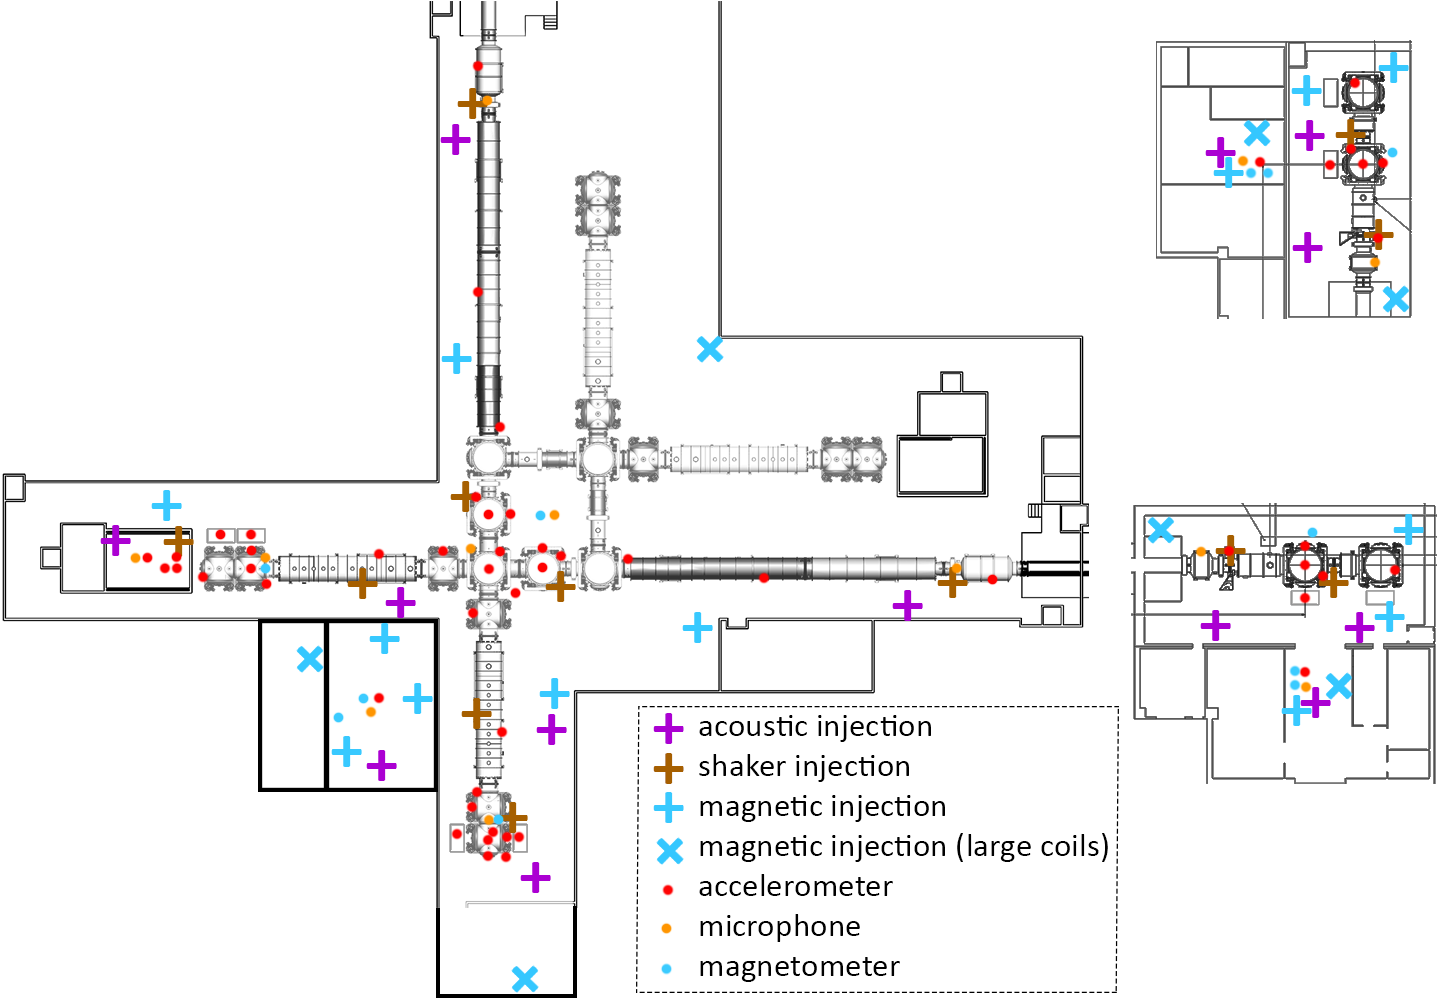
\includegraphics[width=\textwidth]{figures/injection-map.png}
	\caption{
		Standard locations for vibration and magnetic injections at the LHO corner station (left), Y end station (top right), and X end stations (bottom right).}
	\label{fig:injection_map}
\end{figure}

\begin{figure}[h!]
	\centering
	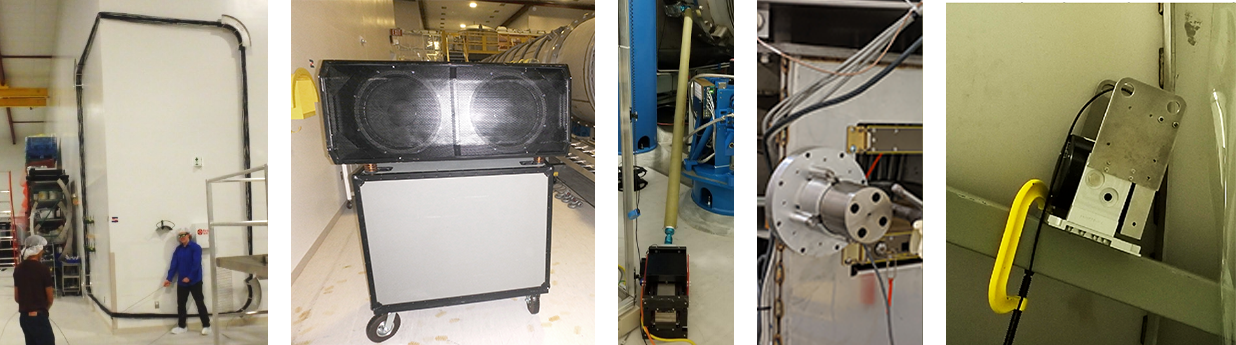
\includegraphics[width=\textwidth]{figures/injection-equipment.png}
	\caption{Injection equipment photos. From left to right: wall-mounted magnetic field injection coil; 14-in. speakers; APS 113 shaker connected to the door of a vacuum chamber by a rigid fiberglass rod; modified Piezosystem shaker clamped to an electronics rack; modified B\&K shaker clamped to a beam tube support.}
	\label{fig:injection_equipment}
\end{figure}


\begin{figure}[h!]
	\centering
	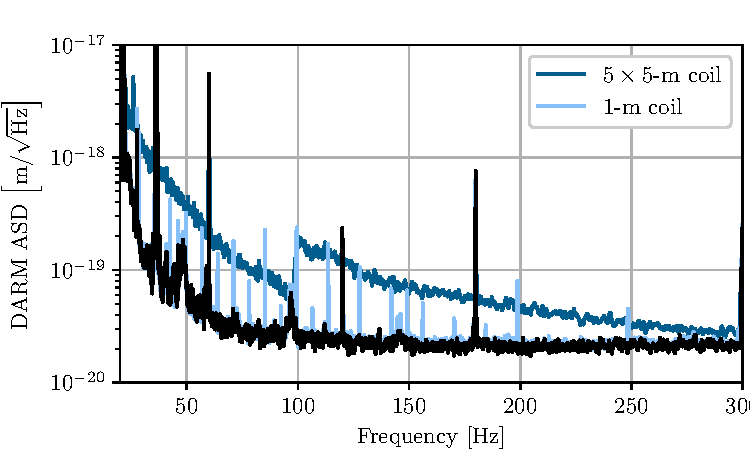
\includegraphics{figures/injection-wallcoil.pdf}
	\caption{
		Comparison of the old small-coil comb magnetic field injections with the new large-coil broadband injections.}
	\label{fig:injection_wallcoil}
\end{figure}

\begin{figure}
	% \includegraphics{figures/injection-cartoon.pdf}
	\caption{
		Illustration of an injection signal propagating to an auxiliary sensor and a coupling site.
		For distant injection sources, the small-angle approximation allows us to treat a sensor near a coupling site as a witness of the noise that couples into the interferometer.}
	\label{fig:injection_cartoon}
\end{figure}

\begin{figure}
	% \includegraphics{figures/injection-cartoon-extended.pdf}
	\caption{
		Illustration of multiple subsequent injections, auxiliary sensors, and coupling sites.}
	\label{fig:injection_cartoon_extended}
\end{figure}

\begin{figure}
	\centering
	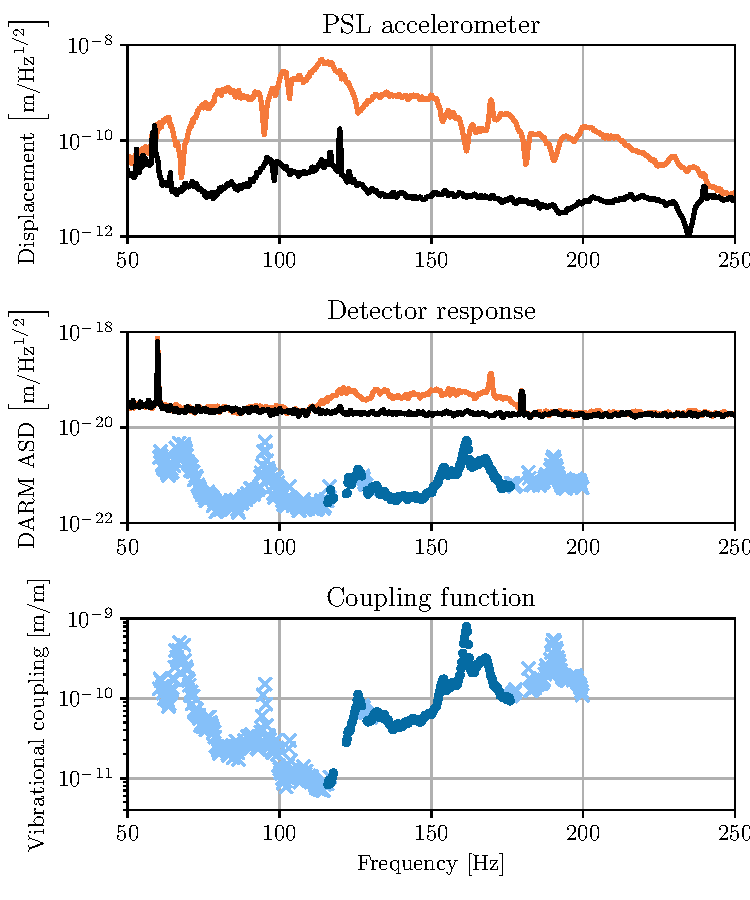
\includegraphics[width=\textwidth]{figures/cf-example.pdf}
	\caption{
		Example of a broadband acoustic noise injection and measurement of a single-injection coupling function.
		Top: displacement of an accelerometer in the PSL room during background time (black) and injection time (orange).
		Middle: DARM during background time (black) and injection time (orange).
		Estimated ambient levels for the accelerometer are shown as dark blue dots, with upper limits shown as light blue crosses.
		Bottom: single-injection coupling function used to produce estimated ambient above.}
	\label{fig:cf_example}
\end{figure}

\begin{figure}[h!]
	\centering
	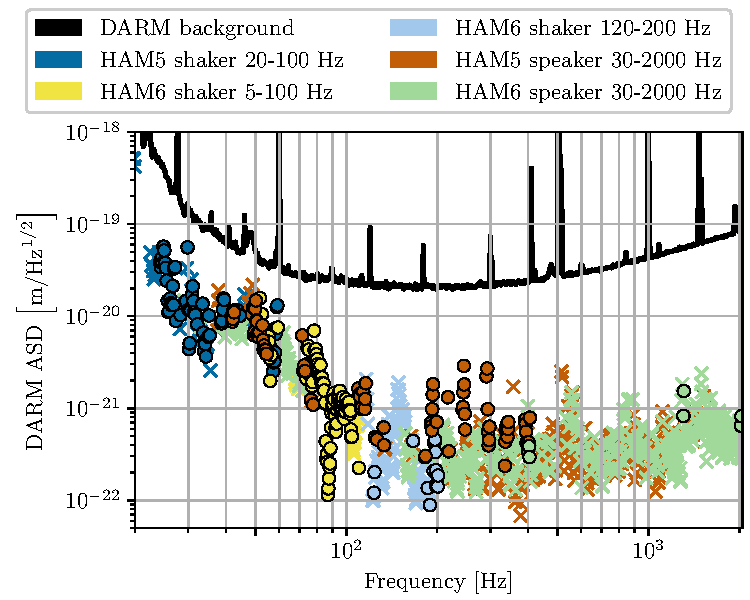
\includegraphics{figures/composite.pdf}
	\caption{
		Ambient noise level for the LHO HAM6 Y-axis accelerometer estimated from a composite coupling function, using acoustic and seismic injections near the output arm.}
	\label{fig:cf_composite}
\end{figure}

\begin{figure}[h!]
	\centering
	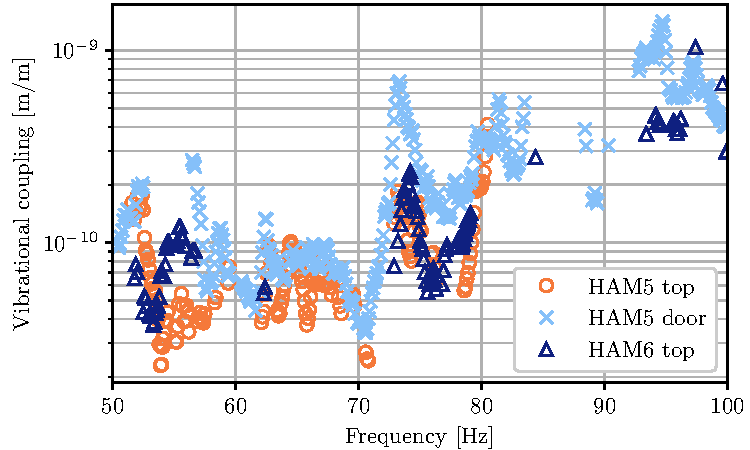
\includegraphics[width=\textwidth]{figures/cf-locations-vib.pdf}
	\caption{
		Single-injection coupling functions (upper limits not shown) for the HAM5 Y-axis accelerometer for three different shaker injection locations (on top of HAM5, on top of HAM6, and on the HAM5 chamber door).}
	\label{fig:cf_locations_vib}
\end{figure}

\begin{figure}[h!]
	\centering
%	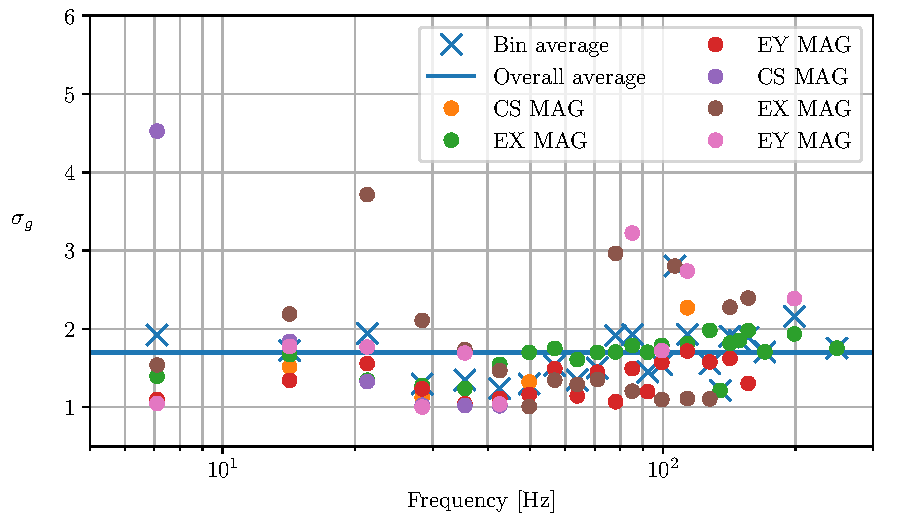
\includegraphics[width=\textwidth]{figures/cf-locations-mag.pdf}
	\caption{
		Single-injection coupling functions (upper limits not shown) for various magnetometers and various injections at both observatories.}
	\label{fig:cf_locations_mag}
\end{figure}

\begin{figure}[h!]
	\centering
	% \includegraphics[width=\textwidth]{figures/smoothing.pdf}
	\caption{
		Applying spectral smoothing to the injection signal recorded by a microphone.
		Smoothing eliminates physical artifacts from the acoustic injection technique, recovering the expected broadband input signal.}
	\label{fig:cf_smoothing}
\end{figure}

\section{Chapter 4}

\begin{figure}[h!]
	\centering
	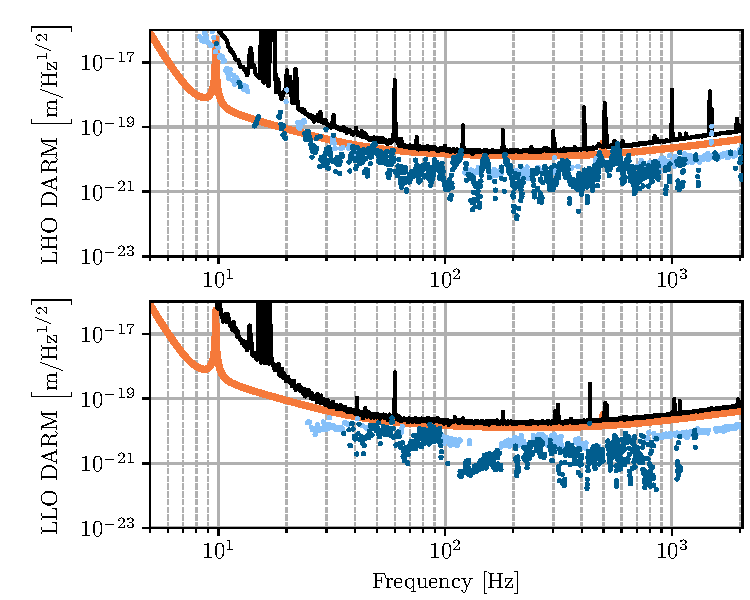
\includegraphics[width=\textwidth]{figures/ambient_vib.pdf}
	\caption{
		Ambient estimate of vibrational noise levels at LHO (top) and LLO (bottom).}
	\label{fig:ambient-vib}
\end{figure}

\begin{figure}[h!]
	\centering
	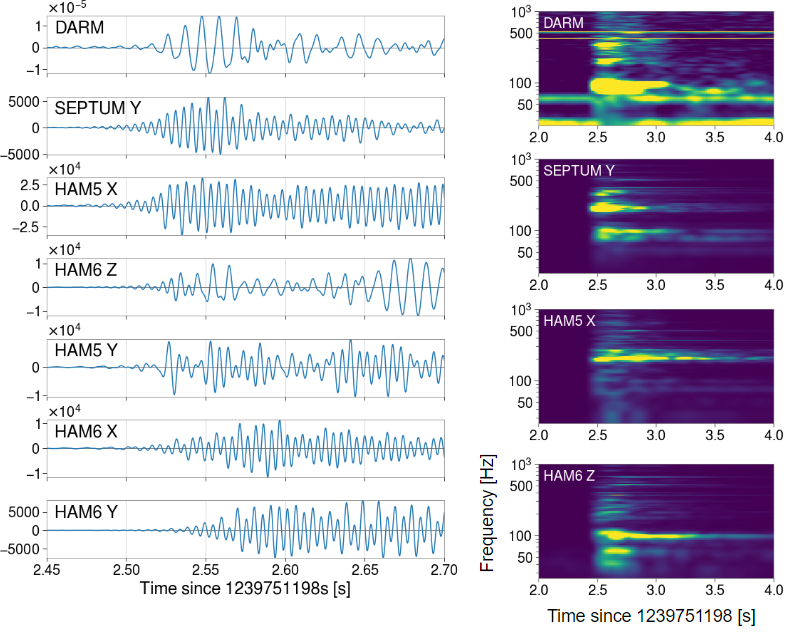
\includegraphics[width=\textwidth]{figures/impulse.png}
	\caption{
		Time series (left) and spectrograms (right) of a vibrational impulse injection produced at the output arm of the LHO detector.}
	\label{fig:impulse}
\end{figure}

\begin{figure}[h!]
	\centering
	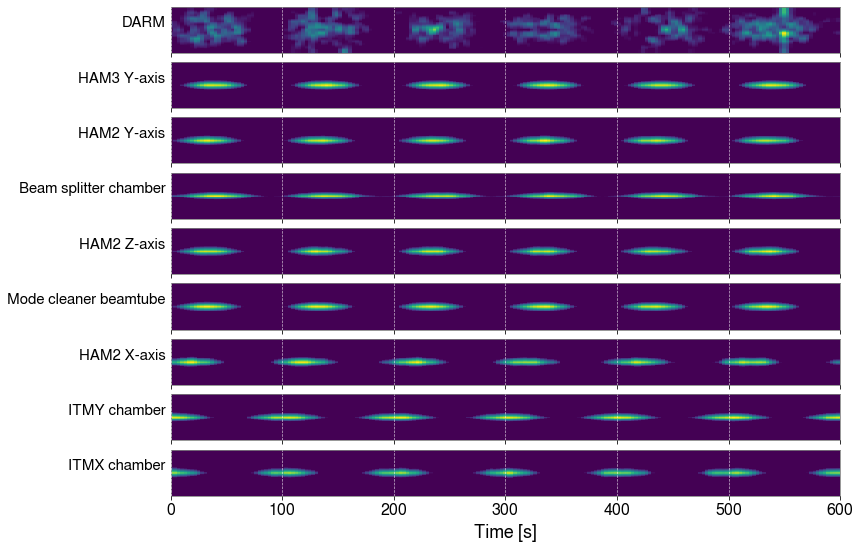
\includegraphics[width=\textwidth]{figures/beat-spectrograms.png}
	\caption{
		Spectrograms of DARM and various accelerometers near the input arm and beam splitter showing a beating-shakers injection at 48\,Hz.}
	\label{fig:beats}
\end{figure}

\begin{figure}
	\centering
	\includegraphics[width=\textwidth]{figures/48Hz.png}
	\caption{LHO DARM spectrum before and after mitigation of the 48-Hz peak.}
	\label{fig:48hz}
\end{figure}

\begin{figure}
	\centering
%	\includegraphics[width=\textwidth]{}
	\caption{Improvement in jitter coupling at LHO (left) and LLO (right) between the start and end of O3.}
	\label{fig:jitter}
\end{figure}

\begin{figure}[h]
	\centering
	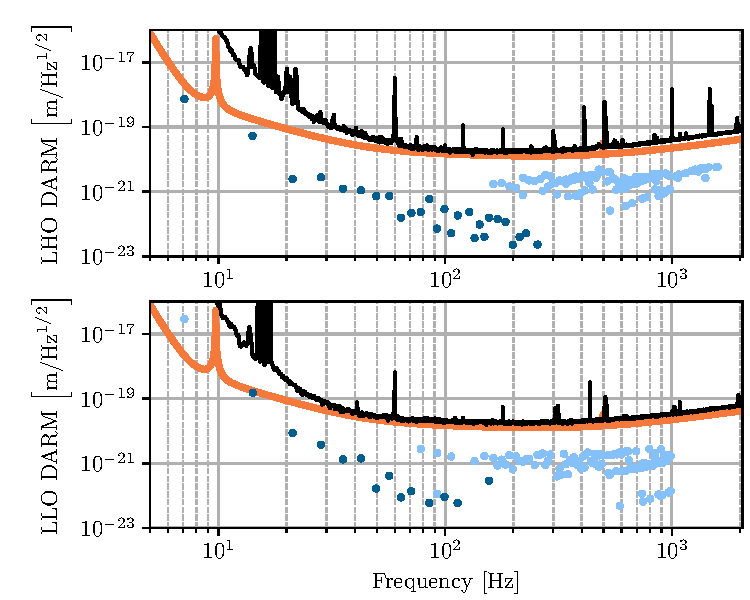
\includegraphics[width=\textwidth]{figures/ambient_mag.pdf}
	\caption{
		Ambient estimate of magnetic noise levels at LHO during March 2019 (blue), prior to O3, and during April 2019 (orange), after O3.}
	\label{fig:ambient-mag}
\end{figure}

\begin{figure}
	\centering
%	\includegraphics[width=\textwidth]{}
	\caption{
		Ambient estimate of magnetic noise levels at LHO during March 2019 (blue), prior to O3, and during April 2019 (orange), after O3.}
	\label{fig:weekly-mag-preO3}
\end{figure}

\begin{figure}
	\centering
%	\includegraphics[width=\textwidth]{}
	\caption{Weekly trends in frequency (top) and amplitude (top) of peaks in the magnetic coupling functions.}
	\label{fig:weekly-mag-variation}
\end{figure}

\begin{figure}
	\centering
%	\includegraphics[width=\textwidth]{}
	\caption{Constant-Q spectrogram of GW170817.}
	\label{fig:vetting_gw170817_spectrogram}
\end{figure}

\begin{figure}
	\centering
%	\includegraphics[width=\textwidth]{}
	\caption{Constant-Q spectrogram of an accelerometer on the PSL table (top) and ambient magnetic noise levels for the same magnetometer (bottom).}
	\label{fig:vetting_gw170817_lho}
\end{figure}

\begin{figure}
	\centering
%	\includegraphics[width=\textwidth]{}
	\caption{Constant-Q spectrogram of an accelerometer on the LLO ETMY chamber (top) and ambient magnetic noise levels for the same accelerometer (bottom).}
	\label{fig:vetting_gw170817_llo}
\end{figure}

\section{Chapter 5}








\end{document}
